%% PRL version distilled from the PRX-scale non-normality manuscript.
%% Core message:
%%   state-dependent gain can reroute perturbations through fixed anatomy, while
%%   a stationary fluctuation budget constrains which response geometry can
%%   dominate. Flexible computation therefore need not require rewiring or a
%%   global approach to spectral criticality.

\documentclass[
  aps,prl,reprint,superscriptaddress,nofootinbib,longbibliography,floatfix,
  amsmath,amssymb
]{revtex4-2}

\usepackage[utf8]{inputenc}
\usepackage[T1]{fontenc}
\usepackage{graphicx}
\usepackage{bm}
\usepackage{placeins}
\usepackage{hyperref}
\hypersetup{hidelinks}

\newcommand{\Tr}{\mathrm{Tr}}
\newcommand{\Rey}{\mathrm{Re}}
\newcommand{\Gmax}{G_{\max}^{(2)}}
\newcommand{\Cnoise}{\mathcal C}
\newcommand{\Rtask}{\mathcal R}
\newcommand{\opnorm}[1]{\left\lVert #1\right\rVert_2}
\newcommand{\frobnorm}[1]{\left\lVert #1\right\rVert_F}

\begin{document}

\title{Flexible neural routing through fluctuation-constrained response geometry}

\author{Mingyi Huang}
\affiliation{Research Institute of Intelligent and Complex Systems, State Key
Laboratory of Medical Neurobiology and MOE Frontiers Center for Brain Science,
and Institute of Science and Technology for Brain-Inspired Intelligence,
Fudan University, Shanghai 200433, China}
\affiliation{Shanghai Artificial Intelligence Laboratory, Shanghai 200232,
China}

\author{Yuguo Yu}
\email{yuyuguo@fudan.edu.cn}
\affiliation{Research Institute of Intelligent and Complex Systems, State Key
Laboratory of Medical Neurobiology and MOE Frontiers Center for Brain Science,
and Institute of Science and Technology for Brain-Inspired Intelligence,
Fudan University, Shanghai 200433, China}
\affiliation{Shanghai Artificial Intelligence Laboratory, Shanghai 200232,
China}

\date{\today}

\begin{abstract}
Critical dynamics explain long timescales; flexible computation requires
a rule for which input a stable circuit routes to which output.  Gain rotates
singular response geometry on fixed anatomy, while fluctuations price
amplification.  Above onset, an exact fixed-spectrum class concentrates
budget into one channel; under isotropic drive, a single pair-supported channel
in any stable real spectrum has onset cost $2/(a_i+a_k)$.  FlyWire and
multi-mouse perturbations support anatomical feasibility and spectrum
insufficiency, yielding a falsifiable routing framework at fixed decay rates.
\end{abstract}

\maketitle

Animals can map the same sensory evidence to different actions as context
changes, even though recurrent anatomy is fixed and ongoing activity must
remain stable~\cite{mante2013context}.  This poses a circuit-level problem: how
can one stable population rapidly reconfigure input--output routing without
rewiring, approaching global instability, or indiscriminately amplifying
background fluctuations?  Neuronal gain changes quickly enough to act as a
control~\cite{ferguson2020gain}, but control alone does not explain which route
is favored.

Recent critical-initialization theory offers a complementary account of
macroscopic spontaneous activity.  Pachitariu \emph{et al.}\ linked power-law
covariance spectra and near-real dynamic-mode-decomposition (DMD) modes to
critically normalized symmetric random dynamics, and showed that this fixed
scaffold supports time-dependent and zero-shot memory through a trained
readout~\cite{pachitariu2026critical}.  This explains long timescales and memory
while explicitly leaving open whether different dynamics are recruited during
task execution.  We address that open computational layer: how a state change
selects which input reaches which output.

We propose singular input--output response geometry as the rapidly
reconfigurable computational state.  For $J_s=-aI+G_sW$, heterogeneous gain
reshapes this geometry on fixed anatomy, whereas stationary propagated variance
prices the resulting routes.  The paper separates three questions:
\emph{identifiability}, whether spontaneous summaries determine the response
map; \emph{controllability}, whether gain can rotate that map on fixed anatomy;
and \emph{selection}, which accessible map is favored at fixed spectrum and
fluctuation budget.  Fixed-anatomy and whole-connectome constructions address
controllability, exact theory gives a finite-budget result in a solvable class
and a pair-supported onset law for arbitrary stable real-eigenvalue spectra,
and multi-mouse perturbations test identifiability.  Critical dynamics may
therefore provide a stable, long-memory scaffold while
fluctuation-constrained response geometry supplies selective routing.

Gain modulation can reorganize activity on fixed anatomy~\cite{stroud2018},
and population gating can select task-relevant routes~\cite{barbosa2023}, while hidden-feedforward memory, balanced
amplification, and non-normal transient coding show that stable directed
dynamics can generate selective transients without slow eigenmodes
~\cite{ganguli2008,goldman2009,murphy2009,hennequin2012,hennequin2014,bondanelli2020}.
These works establish accessibility and amplification; our new element is the
resource rule that compares response geometries at fixed spectrum and
stationary fluctuation cost.  This also differs from fixed-spectrum
expressivity~\cite{kerg2019} and coding optimization against a spiking
cost~\cite{pratcarrabin2026}.  Flexible routing is the phenomenon, response
geometry the computational state, gain the control, and the fluctuation budget
the selection constraint (Fig.~\ref{fig:story}).

\begin{figure*}[t]
  \centering
  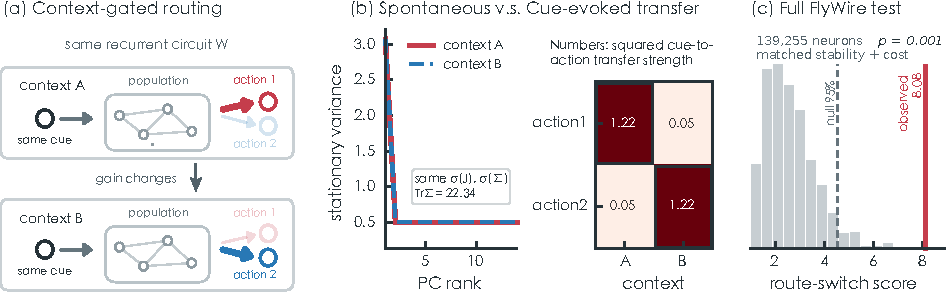
\includegraphics[width=\textwidth]{figures/fig_gain_routing_submission.pdf}
  \caption{\textbf{Matched spontaneous summaries can conceal switched computation.}
  \textbf{(a)} The same sensory cue enters one fixed recurrent circuit $W$.
  Context A uses gain to route it toward action/readout 1, whereas context B
  routes the identical cue toward action/readout 2; no rewiring occurs.
  \textbf{(b, left)}
  The contexts nevertheless match in decay and stationary-covariance spectra,
  total fluctuation cost, and global peak response.  \textbf{(b, right)}
  Perturbation reveals the switched map: output preference changes $25$-fold
  and the routed output direction rotates by $67^\circ$.  \textbf{(c)} An
  analogous gain intervention on two anatomically supported behavioral
  corridors in the full $139{,}255$-neuron FlyWire graph produces a route-switch
  score---the geometric mean of the two within-route selectivity ratios---that
  exceeds the 95th percentile of 999 stratified nulls
  ($p=0.001$) at matched stability and estimated finite-horizon cost.  The gain fields are in silico
  interventions, not measured brain states.}
  \label{fig:story}
\end{figure*}

Figure~\ref{fig:story} establishes the hidden-state and control links, not
selection: gain switches the route at matched spontaneous summaries and global
response capacity, while the v783 analysis shows compatibility with realistic
directed anatomy~\cite{shiu2024,dorkenwald2024,suppl}.  Once a geometry is
accessible, selection begins by treating $\Tr\Sigma$, the white-noise
state-output $\mathcal H_2$ energy, as an effective-dynamics resource rather
than a detailed metabolic model~\cite{attwell2001,hennequin2012,suppl}.  For a
stable generator $J$ driven by background covariance $Q$,
\begin{equation}
  \begin{aligned}
  J\Sigma+\Sigma J^\top+Q=0,
  \qquad
  \Cnoise_Q(J)=\Tr\Sigma
  \\
  =\int_0^\infty \frobnorm{e^{Jt}Q^{1/2}}^2\,dt ,
  \end{aligned}
  \label{eq:cost}
\end{equation}
which defines the stationary cost.  Task response is
$\Rtask_{B,C}(J)=\sup_{t\ge0}\opnorm{Ce^{Jt}B}^2$ and global squared gain is
$\Gmax(J)=\sup_{t\ge0}\opnorm{e^{Jt}}^2$.

The construction holds $W$ fixed and uses two diagonal gain fields to exchange
the strong output branch.  The contexts match in decay and covariance spectra,
total cost, and global peak squared gain, yet cue transfer changes $25$-fold and the
output rotates by $67^\circ$.  Matching spontaneous summaries and scalar
responsiveness therefore does not identify which downstream population receives
the input.

On the full $139{,}255$-neuron FlyWire graph, matched diagonal gain fields gave
a route-switch score of $8.08$, above a stratified-null $95\%$ bound of $3.10$
($p=0.001$, 999 permutations), at matched spectral radius and estimated
finite-horizon cost (Supplemental Material).  This does not show that the fly uses these gain
fields; it shows that complete anatomy supplies the required directed degrees
of freedom.

These quantities separate decay, spontaneous variance, and finite-time routing.
Matching the first two need not match computation.  Equation~\eqref{eq:cost}
charges a route by the ongoing variability it creates, converting response
geometry into a physical allocation problem.

The dynamical mechanism now becomes relevant.  Every stable normal generator
is contractive, $\Gmax=1$; amplification at fixed negative spectral abscissa
therefore requires non-normal response geometry.  We first solve a deliberately
minimal fixed-spectrum feedforward class
\begin{equation}
  J=-aI+K,\qquad a>0,\qquad K^2=0,
  \qquad \lambda_i(J)=-a .
  \label{eq:squarezero}
\end{equation}
which transfers activity between orthogonal subspaces without feedback and
leaves every eigenvalue fixed.  Let $s_1\ge\cdots\ge s_r>0$ be the nonzero
singular values of $K$; then $e^{Jt}=e^{-at}(I+tK)$ exactly.

For isotropic ongoing drive, $Q=I$, solving Eq.~\eqref{eq:cost} gives
\begin{equation}
  \Cnoise_I(J)=\frac{N}{2a}
  +\frac{\frobnorm{K}^2}{4a^3}
  =\frac{N}{2a}+\frac{\sum_i s_i^2}{4a^3}.
  \label{eq:costexact}
\end{equation}
Thus stationary cost fixes the total squared singular strength, whereas exact
peak squared gain depends only on the largest singular value $s_1$ (Supplemental
Material).  Since $s_1^2\le\sum_i s_i^2$, the fixed-cost maximizer is
\begin{equation}
  K_\star=s_\star uv^\top,\quad u^\top v=0,\quad
  s_\star=\sqrt{4a^3(C_0-C_{\rm normal})}.
  \label{eq:rankone}
\end{equation}
where $C_{\rm normal}=N/(2a)$ and $u,v$ are unit singular vectors.  This is the response-allocation principle:
a matched fluctuation budget is best concentrated into one dominant directed
mode (rank one only in this solvable limit).  Above amplification onset the
ranking is strict; below it all allocations are contractive.  Proofs and
degenerate cases are given in the Supplemental Material~\cite{suppl}.

The concentration has a direct neural interpretation but is not a claim of
rank-one anatomical connectivity.  A distributed circuit may contain many
recurrent pathways; the result concerns its effective finite-time response.
For a fixed total fluctuation penalty, spreading coupling over several
orthogonal channels charges every channel through
$\sum_i s_i^2$, whereas the strongest task response can use only the largest
$s_i$.  Concentration therefore creates response specialization: one input can
be strongly routed while the remaining directions stay stable and relatively
quiet.  This differs from globally increasing susceptibility, which enhances
many directions while lengthening their decay.

Amplification begins at excess cost $\Delta C_\star=1/a$ without moving any
eigenvalue or slowing relaxation.  Its fractional cost is $2/N$ of the normal
baseline, but its absolute cost remains finite; the durable result is therefore
the concentrated allocation, not a ``free'' large-network threshold.

\begin{figure}[!b]
  \centering
  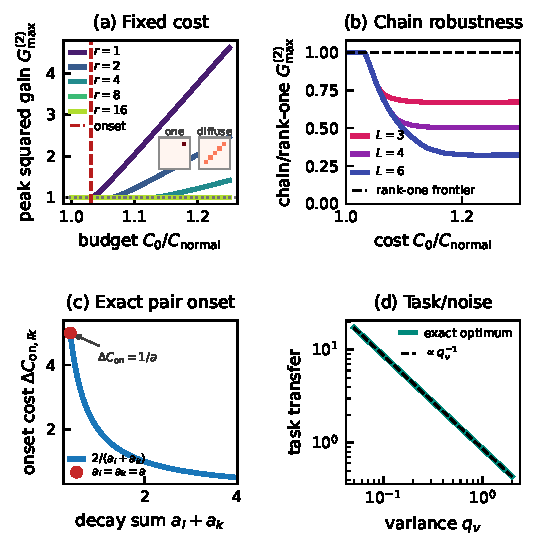
\includegraphics[width=\columnwidth]{figures/fig_fixed_budget_selection.pdf}
  \caption{\textbf{Fluctuation cost shapes response geometry.}
  \textbf{(a)} In the equal-decay square-zero class, concentrating a matched
  budget into one channel crosses amplification while diffuse allocations remain
  contractive; inset, the corresponding geometries.  \textbf{(b)} Tested
  higher-order chains remain below this finite-budget frontier.  \textbf{(c)} A
  single pair-supported channel, as the only nonzero Schur coupling embedded in
  any stable real-eigenvalue spectrum, obeys
  an exact onset law; the marker is the equal-decay limit used in (a).
  \textbf{(d)} Under the stated cross-term condition, structured background
  drive favors task-relevant directions with low ongoing variance.}
  \label{fig:fixedbudget}
\end{figure}

An exact unequal-decay result extends the onset calculation.  For one ordered
Schur-mode pair of a stable real-eigenvalue spectrum,
\begin{equation}
  J_{ik}=\begin{pmatrix}-a_i&m\\0&-a_k\end{pmatrix},
  \qquad a_i,a_k>0,
  \label{eq:pairgenerator}
\end{equation}
is spectrum preserving.  Under isotropic drive its stationary excess cost is
exactly $m^2/[2a_i a_k(a_i+a_k)]$, while transient-growth onset occurs at
$m^2=4a_i a_k$.  Hence
\begin{equation}
  \Delta C_{{\rm on},ik}=\frac{2}{a_i+a_k}.
  \label{eq:paironset}
\end{equation}
This finite-coupling result is exact.  Onset cost is set by $a_i+a_k$, whereas
the required coupling magnitude is $2\sqrt{a_i a_k}$; increasing both decay
rates therefore lowers integrated cost while requiring stronger coupling.  The equal-decay case $a_i=a_k=a$
recovers $1/a$.  For distributed Schur coupling, by contrast, the weighted
quadratic cost is local; its generic finite-amplitude threshold and
finite-budget optimum remain open~\cite{suppl}.

Structured drive selects the orientation of the channel.  Let
$K=suv^\top$, $\|u\|=\|v\|=1$, $u^\top v=0$, and suppose the anisotropic-cost cross term
$u^\top Qv$ vanishes; $Qv=q_vv$ is one sufficient condition.  The directed
transfer peaks at $t=1/a$, and eliminating channel strength gives
\begin{equation}
  \frac{\Rtask_{v,u}}
  {\Cnoise_Q-\Tr Q/(2a)}
  =\frac{4a}{e^2q_v}.
  \label{eq:efficiency}
\end{equation}
At fixed excess cost in this reduced problem, efficient channels favor high
task relevance and low background variance.  With $Q$ positive definite on
the feasible input subspace, the multidirectional quadratic reduction gives
generalized eigenvectors $Rv=\lambda Qv$ under the feasibility
conditions in the Supplemental Material~\cite{suppl}; when the cross term
cannot be removed, orientation depends jointly on input and output directions.
Thus the reduced rule has a whitening form without asserting a universal
whitening prescription for arbitrary anisotropic dynamics.

This orientation rule gives the allocation principle computational content.
If two candidate inputs are equally relevant but one lies along a direction of
large ongoing variance, amplifying it incurs a larger stationary penalty.
A task-relevant direction quiet at baseline can instead receive transient gain
without making the whole population broadly excitable.  Attention or state can
therefore reorient a channel through gain, while background covariance prices
each orientation.  The prediction concerns a concentrated task-evoked map, not
globally low-dimensional activity.

For distributed Schur coupling, the local weighted-cost functional can select
a dense emergent direction, so infinitesimal onset and finite-budget
optimization need not select the same architecture.  Only for $K^2=0$ do
higher-order costs vanish and make concentration exactly optimal; matched-cost
tests of higher-order chains remain below that frontier
[Fig.~\ref{fig:fixedbudget}(b)] but do not prove global optimality
~\cite{suppl}.

\begin{figure*}[t]
  \centering
  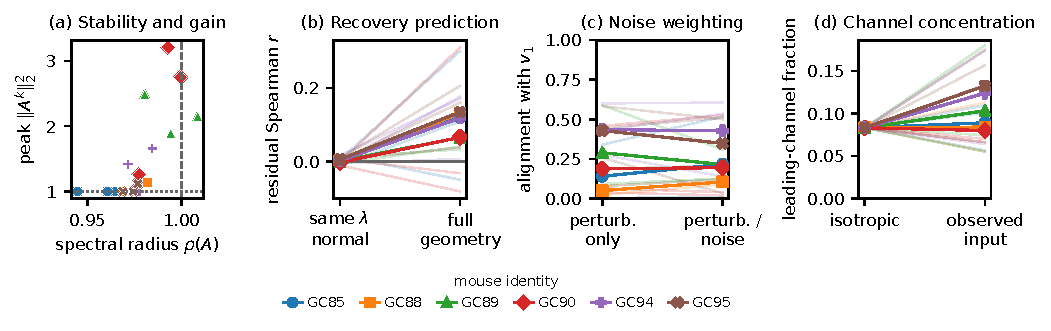
\includegraphics[width=\textwidth]{figures/fig_alm_main.pdf}
  \caption{\textbf{Multi-mouse photoinhibition tests the spectrum-insufficiency premise.}
  Seventeen bilateral-ALM sessions represent six mice
  ~\cite{chen2021modularity,chenli2022dataset}.  \textbf{(a)} Fitted stability
  and gain are descriptive; colors and markers identify mice throughout.  \textbf{(b)} Full
  geometry predicts recovery better than the median randomly oriented,
  exact same-spectrum normal control in all mice.  \textbf{(c)} The ordering persists across latent dimensions.
  \textbf{(d)} It remains positive in five of six mice after stricter condition
  adjustment.  This tests information beyond the spectrum, not biological
  budget optimality.}
  \label{fig:empirical}
\end{figure*}

The data test a narrower premise: does response geometry contain recovery
information that the eigenvalue spectrum omits?  Seventeen of the 18
individually exposed bilateral-ALM session files passed outcome-independent gates and represented six
mice~\cite{chen2021modularity,chenli2022dataset,suppl}.  Operators fit only to
control trials outperformed the median of 200 randomly oriented exact
same-spectrum normal controls in every mouse
(paired median difference $0.117$; $p=0.0156$, the minimum exact one-sided value
for $n=6$), with the ordering preserved across latent dimensions.  Exploratory
task/noise weighting was negative (three of six mice; $p=0.656$), so orientation
remains prospective.  The experiment supports spectrum insufficiency, not
gain-mediated rerouting or biological budget optimization.

Each normal surrogate preserves the fitted eigenvalues exactly while replacing
the singular orientation.  The full operator's advantage over the typical
randomly oriented control therefore cannot be attributed to different linear
relaxation times; it does not exclude an optimally fitted normal response
model.  The advantage survives latent dimensions 8, 12, and
16 and condition adjustment in five of six animals
[Fig.~\ref{fig:empirical}(c),(d)].  It concerns trajectories following a causal
photoinhibitory displacement, supporting spectrum insufficiency across animals;
the negative orientation test precludes a claim of task/noise optimality.

The evidence has non-interchangeable roles: the construction shows distinct
maps on one fixed circuit, FlyWire tests anatomical compatibility, the model
supplies selection once fluctuations are charged, and photoinhibition tests for
recovery information beyond the spectrum.  Together they trace anatomical
possibility to observable response geometry, leaving adaptive selection for a
targeted experiment.

Relative to critical initialization~\cite{pachitariu2026critical}, we ask what
computational degree of freedom remains after spontaneous spectra and timescales
are matched: the input--output map and its state dependence.  Prior work showed
that gain and hidden feedforward or non-normal dynamics can control and amplify
such maps.  We add their stationary price: at matched stable spectrum, which
finite-time response geometry can deliver amplification under a bounded
fluctuation cost?  The exact pair law extends this question beyond a degenerate
spectrum, while the finite-budget theorem identifies concentration on the
cost-truncation locus.  Perturbations identify the route, gain rotates it, and
stationary fluctuations price its capacity.

This distinction changes what should be measured.  A covariance spectrum or a
set of relaxation times can characterize spontaneous state space without
revealing the operative computation; an anatomical graph can list possible
routes without revealing which one gain has activated.  Perturbation experiments
are therefore required to identify the singular input--output map.  Comparing
task states at matched decay and cost tests the selection law: flexible
computation becomes geometric reallocation within a stable circuit, not global
criticality.

The resulting picture complements criticality at a different explanatory
level.  Proximity to a transition can account for long timescales, broad
coordination, and high global susceptibility.  It does not by itself determine
which sensory direction is amplified, where that activity is delivered, or
how the route changes between tasks.  Response geometry supplies that map, and
fluctuation constraints turn it into a resource-allocation problem:
responsiveness is placed selectively rather than raised uniformly.  The same
distinction applies to any stable driven system that must remain quiet in most
directions yet respond strongly in a few.

In summary, flexible routing is the phenomenon, response geometry is its hidden
computational state, gain makes that state controllable, and stationary
fluctuations constrain its allocation.  Exact finite-budget concentration is
limited to the square-zero class; the pair-onset law is exact for a
single-pair-supported channel embedded in any stable real-eigenvalue spectrum,
whereas generic finite-budget
optimization remains open.  FlyWire establishes anatomical compatibility and
ALM establishes information beyond eigenvalues; no data yet show biological
budget optimization.  The direct experiment is to
fit effective dynamics in two task or attention states, select state pairs with
matched decay spectrum and stationary cost, and measure their causal response
maps with patterned perturbations.  The theory predicts rotation of the leading
singular directions toward the task-to-noise mode, stronger task transfer, and
no critical slowing.  Failure of this ordering under perturbation rejects the
mechanism.  Criticality may explain broad coordination;
fluctuation-constrained geometry explains which input a stable circuit routes
to which output.

\begin{acknowledgments}
We thank colleagues for helpful discussions.  OpenAI Codex (GPT-5), Anthropic
Claude Code (Opus 4.8 and Sonnet 5), and OpenAI ChatGPT assisted with code and
manuscript review; the authors directed and independently verified all outputs.
\end{acknowledgments}

\emph{Data and code.---} Public source data are cited above.  Code,
machine-readable outputs, and provenance records are archived at
\url{https://github.com/Mia9469/SSNN/tree/prl-routing-submission-v1/Nature_Work/energy_nonnormal};
large third-party datasets are not redistributed.

% PRL requires references cited only in the Supplemental Material to appear
% in the Letter's reference list as well.
\nocite{zhangabbott2000,semedo2019,costacurta2024,christodoulou2022,
jovanovic2005,hu2022,zavatoneveth2026,wakhloo2026,trefethen2005,
neftci2019,chau2025}
\bibliographystyle{apsrev4-2}
\bibliography{references}

\end{document}
